\usetikzlibrary{arrows.meta,calc,matrix}

\begin{frame}{Linux x86-64 calling convention (1)}
    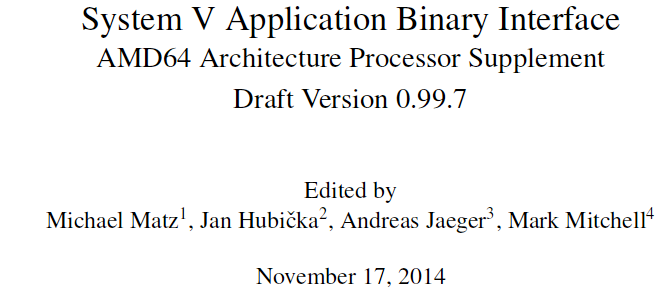
\includegraphics[width=\textwidth]{../asm/sysv-abi-front}
\end{frame}

\begin{frame}{Linux x86-64 calling convention (2)}
    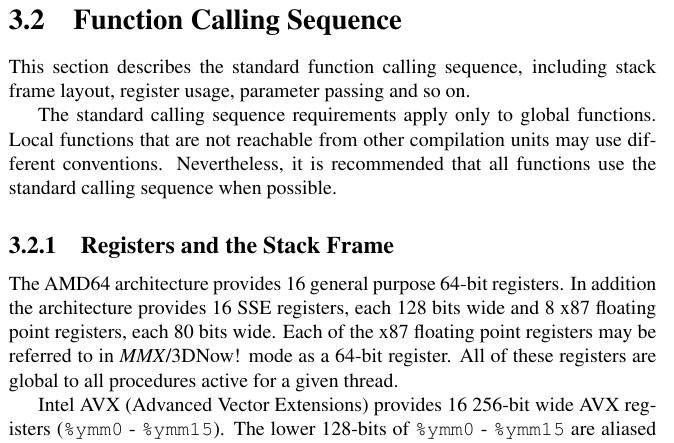
\includegraphics[width=\textwidth]{../asm/func-call-seq-manual}
\end{frame}

\begin{frame}{Linux x86-64 calling summary}
\begin{itemize}
    \item first 6 arguments: \%rdi, \%rsi, \%rdx, \%rcx, \%r8, \%r9
        \begin{itemize}
        \item floating point arguments: \%xmm0, \%xmm1, etc.
        \end{itemize}
    \item additional arguments: push on stack
    \item return address: push on stack
        \begin{itemize}
        \item {\tt call}, {\tt ret} instructions assume this
        \end{itemize}
    \item return value: \%rax
\end{itemize}
\end{frame}



\begin{frame}[fragile,label=conventionEx]{calling convention example}
\begin{lstlisting}[language=C,style=small]
int foo(int a, int b, int c, int d, int e, int f, int g, int h);
...
foo(1, 2, 3, 4, 5, 6, 7, 8);
\end{lstlisting}
\begin{lstlisting}[language=myasm,style=small]
pushq   $8
pushq   $7
movl    $6, %r9d
movl    $5, %r8d
movl    $4, %ecx
movl    $3, %edx
movl    $2, %esi
movl    $1, %edi
call    foo
/* return value in %eax */
\end{lstlisting}
\end{frame}

